\begin{frame}
\frametitle{Introducci\'on}
	\only<1->{
	La din\'amica de los fluidos incompresibles es descrita mediante las siguientes ecuaciones:
	}
	\only<2->{
	\begin{block}{Ecuaciones de Navier-Stokes}	
		\begin{equation*}
		\left \lbrace \begin{array}{ll}
		\nabla \cdot v = 0, \\
		(\rho v)_t + (\nabla \cdot \rho v) v + \nabla p - \mu \nabla^2 v - \rho G = 0.
		\end{array}  \right .
		\label{navierstokes}
		\end{equation*}
		$\rho =$ Densidad, $p =$ Presi\'on, $v =$ Velocidad, $\mu =$ Viscosidad.
	\end{block}
	En este caso, $G$ representa los efectos gravitacionales.
	}
\end{frame}

\begin{frame}
	\only<1->{
	Definiendo $x \in I \subset \mathbb{R}$, y $\alpha = \frac{\mu}{\rho}$; considerando $\rho, p, \mu =$ constantes.
	\begin{block}{Ecuacion de Burgers' (Formulaci\'on Fuerte)}
	\begin{equation*}
	\frac{\partial v(x, t)}{\partial t} +  \underbrace{v(x, t) \frac{\partial v(x, t)}{\partial x}}_{\textbf{Convecci\'on}} - \underbrace{\alpha \frac{\partial^2 v(x, t)}{\partial x^2}}_{\textbf{Difusi\'on}} - \hspace{1mm}g(x, t) = 0.
	\end{equation*}
	\end{block}
	}
	\only<2->{
	\begin{block}{Soluci\'on An\'alitica $(g \equiv 0)$}	
		\begin{equation*}
		v(x, t) =  \displaystyle \frac{\int_{-\infty}^{\infty} \frac{x - \xi}{t} \varphi_0 (\xi) e^{- \frac{(x - \xi)^2}{4 \alpha t}} d\xi}{\int_{-\infty}^{\infty} \varphi_0 (\xi) e^{- \frac{(x - \xi)^2}{4 \alpha t}} d\xi}, \hspace{2mm} \varphi_0 (\xi) = e^{- \int_{0}^{\xi} \frac{v_0 (y)}{2 \alpha} dy} 
		\end{equation*}
	\end{block}	
	}
\end{frame}

\begin{frame}
Condicion inicial $v_0 (x) = e^{-0.05x^2}$ y con $\alpha = 0.01$.
\begin{figure}
	\centering
	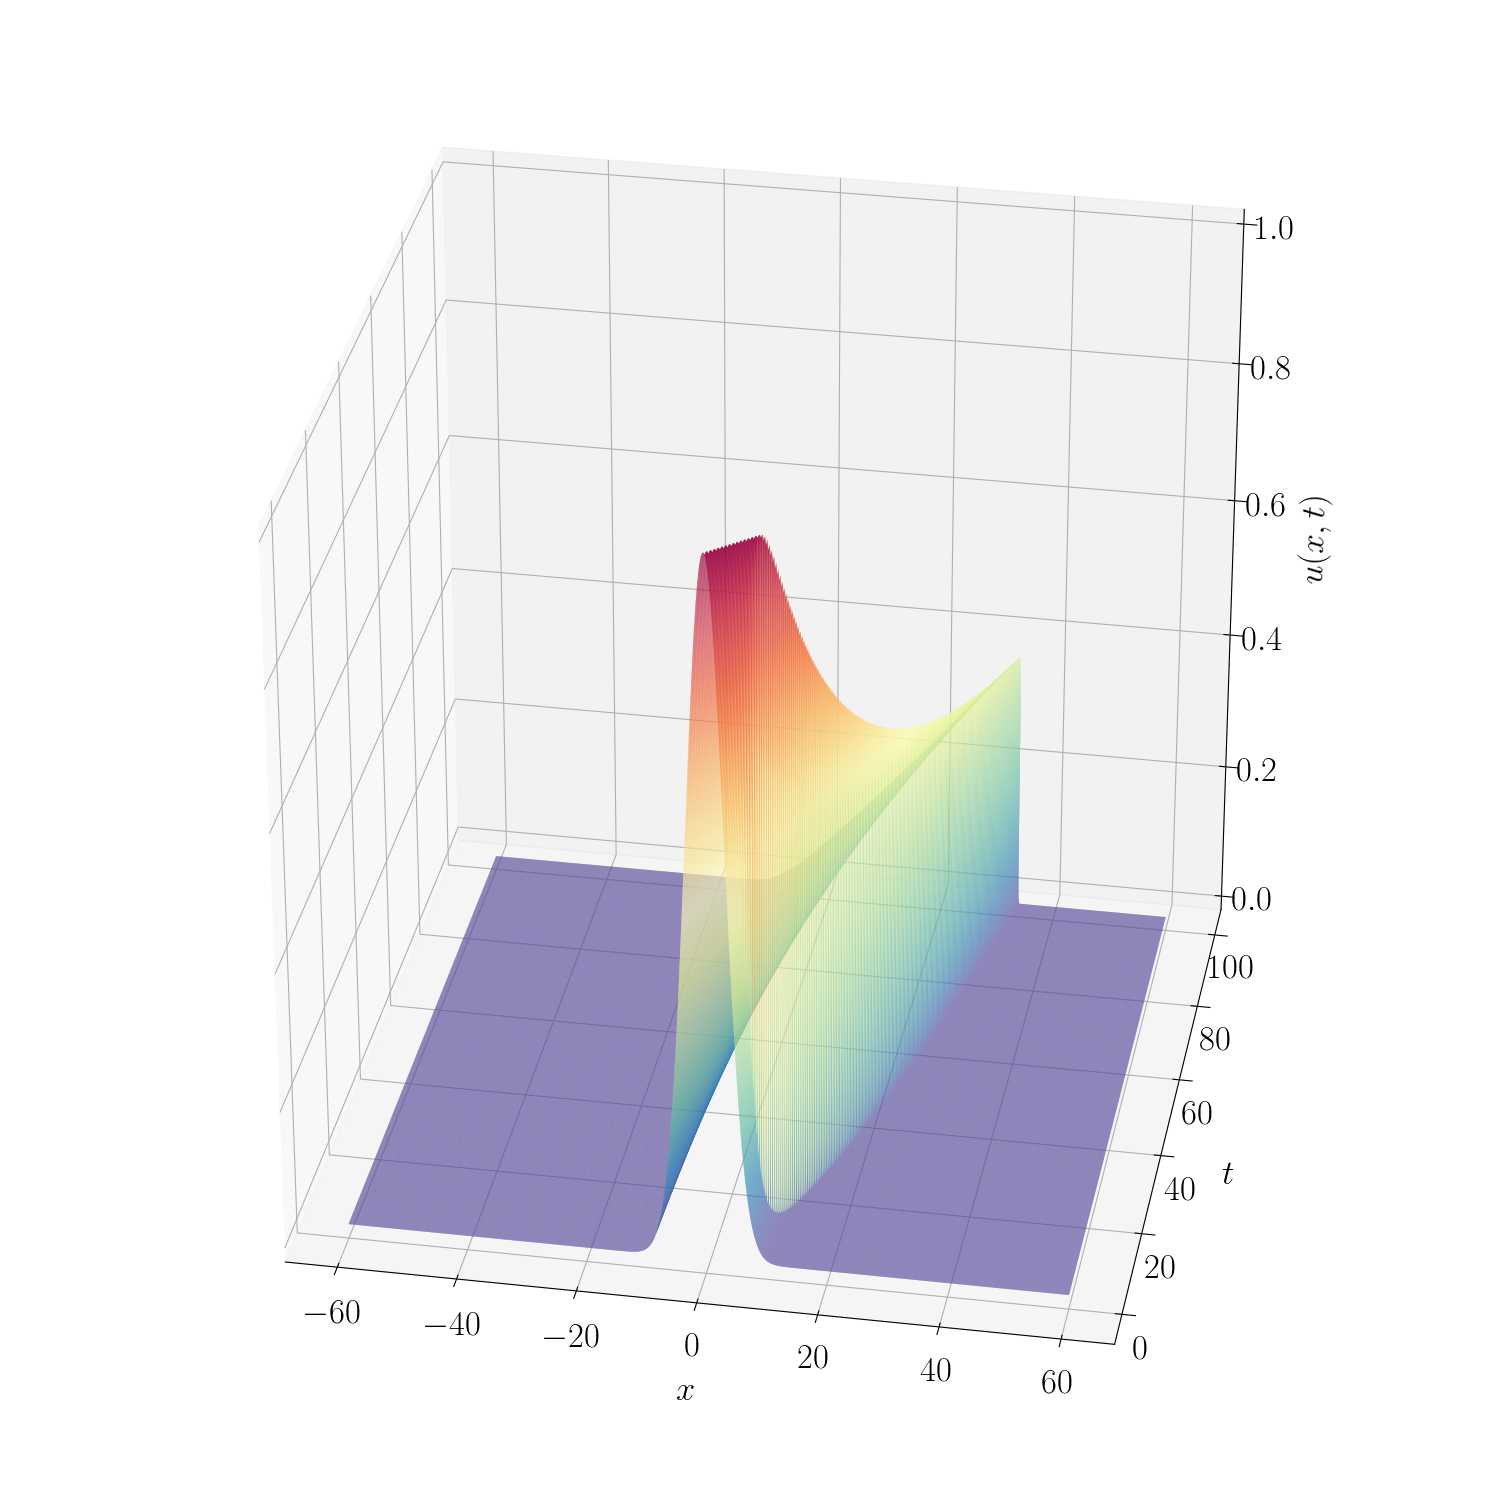
\includegraphics[width=7.5cm]{FIGURES/Galerkin/Graphics/eps=0.01/Exact_Solution_alpha=001.png}
\end{figure}
\end{frame}



\begin{frame}
	%Multiplying both sides of (\ref{strong}) by $\phi \in X$, for some appropriate space $X$ such that the integral of the PDE over the space $I$ is satisfied, we get   
	\only<1->{
	Simplificando notaci\'on:
	\begin{equation*}
	F(t, v) = \frac{1}{2} (v^2)_x - g(x, t), \hspace{3mm} A(v) = - \alpha v_{xx},
	\end{equation*}
		}
		\only<2->{
		\begin{equation*}
		\frac{\partial v}{\partial t} + A(v) + F(t, v) = 0, \hspace{2mm} t > 0.
	\end{equation*}
	}
	\only<3->{
	Con una adecuada elecci\'on de funciones de prueba $\phi \in X$	,
	\begin{block}{Formulaci\'on D\'ebil}	
	\begin{equation*}
	\displaystyle \int_{I} \frac{\partial v}{\partial t} \phi dx + \int_{I} A(v) \phi dx + \int_{I} F(t, v) \phi dx = 0, \hspace{2mm} \forall \phi \in X,\hspace{2mm} \forall t > 0.
	\end{equation*}
	\end{block}
	}
	\only<4->{
	\begin{block}{Formulaci\'on D\'ebil (Compacta)}	
	\begin{equation*}
	\left \langle \frac{\partial v}{\partial t} + A(v) + F(t, v), \phi\right\rangle = 0, \hspace{2mm} \forall \phi \in X, \hspace{2mm} \forall t > 0.
	\end{equation*}
	\end{block}
	}
\end{frame}